
\section{pepe the frog}

\includegraphics [width=.9  \textwidth] {image/frog.jpg}
\begin{figure}
\begin{center}
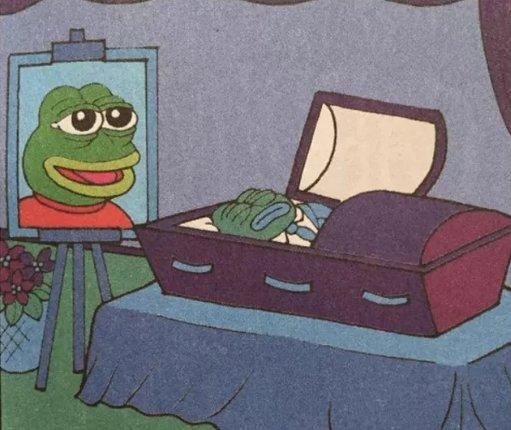
\includegraphics  [width=0.5  \textwidth] {image/frog2.jpg} %ajustement de taille
\end{center}
\caption{sad pepe}
\label{figure zzzz}
\end{figure}
Pepe the Frog’s battles are finally over. Cartoonist Matt Furie has officially killed off his most famous creation, which rose from internet meme to white supremacist mascot during the 2016 US election. As reported by Comic Book Resources, Furie published a one-page installment of his “Boy’s Club” series (where Pepe was first introduced in 2005) in celebration of Free Comic Book Day. The strip shows Pepe laid to rest in an open casket while his friends gather round to mourn. One pours out some whisky for the departed frog, splashing it on Pepe’s face. 
Furie hasn’t spoken about the new cartoon, but its publication seems to bring to an end his quest to rehabilitate Pepe. When the alt-right version of the cartoon became a widespread meme last year, Furie was initially upbeat, saying Pepe’s political affiliation was just “a phase,” and that the cartoon’s “lovable, and charming status will be intact as early as next week.” 
